\if0
☆レポート課題(チームで一部だけ提出して下さい)

1. 表紙(課題名、チームメンバ氏名、提出日)

2. SingleCycleMIPSのモジュール仕様書
 設計した各モジュールについて、上位階層から順に、下記の内容をまとめること。
 ・モジュール名
 ・モジュールの入出力信号名とその説明

例: 入力信号一覧
name 	width 	explanation
CLK 	[0:0] 	SingleCycleMIPS用クロック信号
PC 	[31:0] 	次に実行する命令アドレスを格納するレジスタ値


 ・モジュール内のブロック図(サブモジュール間の接続関係を明示すること。ただし、最下層のIF, ID, EX, MAについては、ブロック図は不要です。)
 ・モジュールの動作の説明文

3. 実機DE10-Liteでの動作検証
 ・テストプログラムのファイル名一覧(load_store, arithmetic, array, if_then_else, while, function, recursion, hanoi)
 ・テストプログラムの実行方法
 ・テストプログラムの検証法
 ・各テストプログラムの検証結果

4. 考察(メンバ一人づつ、個別の考察を記述して下さい。1600文字以上/人)
 ・今回の回路設計で工夫した点(技術的な視点、チーム内での役割分担等のプロジェクト管理的な視点)
 ・より実用的なMIPSプロセッサを実現するために、マイクロアーキテクチャの観点から改良すべき点、および、それに関連して追加で実装すべき機能/回路

5. 感想(メンバ一人づつ、個別の感想を記述して下さい。800文字程度)

6.参考文献
\fi
\documentclass[dvipdfmx]{jsarticle}
\usepackage{graphicx}[dvipdfmx]
\usepackage{multirow}
\usepackage{array}
\usepackage{amsmath,amssymb}
\usepackage{url}
\usepackage{listings}
\usepackage{color}
\usepackage{verbatim}

\title{計算機設計論 レポート課題:MIPSプロセッサの回路設計}
\author{1295149 森岡悠人\\}
\date{\today}

\begin{document}
\maketitle

\section{モジュール仕様書}


QuartusのRTL Viewerを用いて出力した,DE10-liteに書き込んだモジュールのブロック図を図\ref{fig:rtl}に示す.
\begin{figure}[h]
\centering
  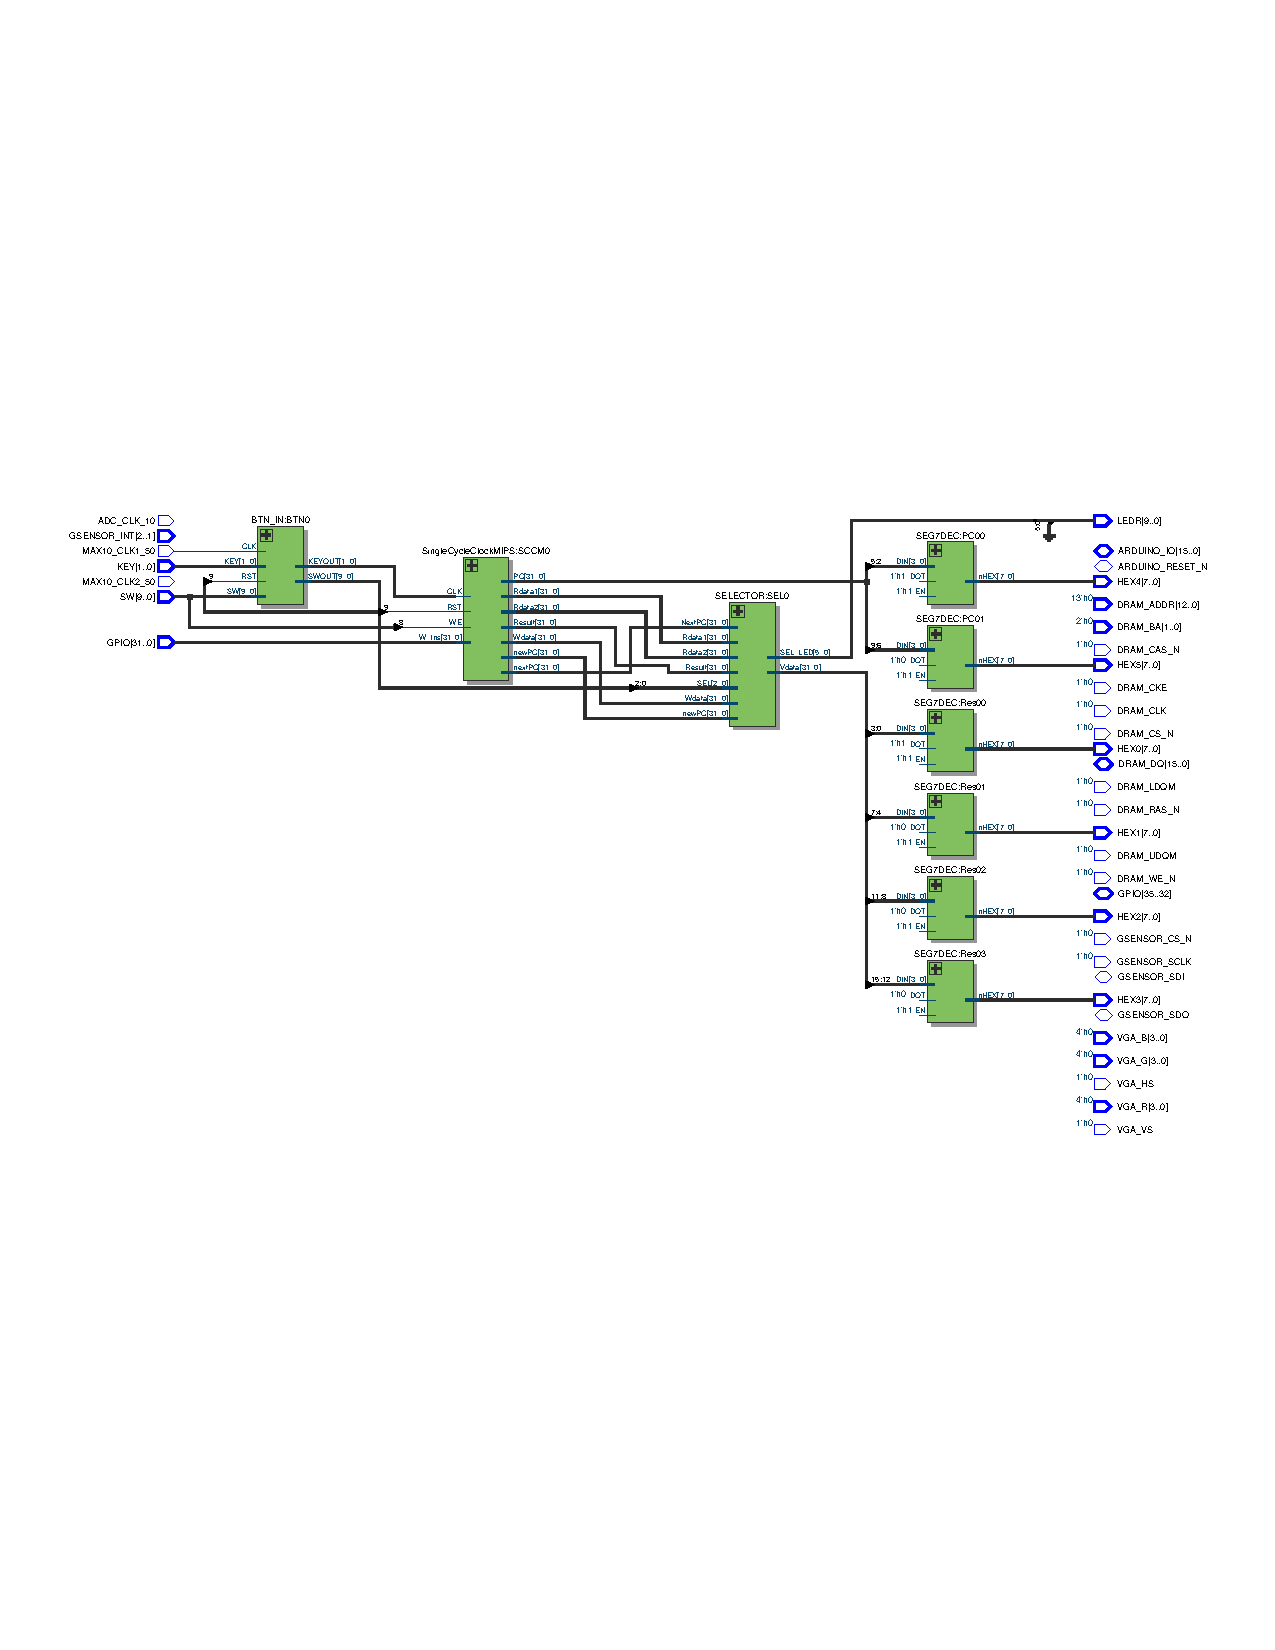
\includegraphics[width=\textwidth]{myRTL.png}
  \caption{作成したMIPS回路のブロック図}
  \label{fig:rtl}
\end{figure}



\section{動作検証}
作成したverilogコードがMIPSの命令セットを実行できるかどうかの検証を行った.
テストプログラムとして,教科書\cite{textbook}に掲載されているアセンブラプログラム(load\_store, arithmetic, array, if\_then\_else, while, function, recursion, hanoi)を用いた.
プログラムはCPUlator MIPS System Simulator \cite{mips-sim}を用いてコンパイルし,32bitの16進数で出力されたバイナリを\texttt{IMem.txt}に書き込んでおき,IMに読み込ませて実行した.
動作の流れとデータメモリの中身を確認するため,modelsim20.1を用いて動作のシミュレーションと検証を行った.
シミュレーション結果は,display命令を用いて,PC, Instruction, ALU\_resultレジスタの順番が期待通りかどうかを確認した.
シミュレーションの様子を図\ref{fig:simulation}に示す.
\begin{figure}[h]
\centering
  \includegraphics[width=0.8\textwidth]{modelsim.png}
  \caption{modelsimによるシミュレーションの様子}
  \label{fig:simulation}
\end{figure}

\subsection{test: load\_store}

\subsubsection{load\_storeのテスト結果}
\verbatiminput{test-results/load_store.txt}

\subsection{test: arithmetic}
あらかじめテストベンチでDMemの0番地からそれぞれ変数a=1,b=2,c=3,d=0と変数のオフセットを保持するレジスタ\$s7=0を初期値として設定してシミュレーションを実行した.
その結果,期待通りa, b, cの値がadd命令で足し合わされ,\$s3=6であることを確認した.
\subsubsection{arithmeticのテスト結果}
\verbatiminput{test-results/arithmetic.txt}

\subsection{test: array}
あらかじめテストベンチでDMemの0番地からそれぞれ配列a[0]=0, a[1]=1..., a[9]=9と配列のオフセットを保持するレジスタ\$s7=0と\$s2=2を初期値として設定してシミュレーションを実行した.
その結果,期待通り\$s1=2, \$s2=5であることを確認した.
\subsubsection{arrayのテスト結果}
\verbatiminput{test-results/array.txt}

\subsection{test: if\_then\_else}
まず,if文が真になる場合のテストを行った.
あらかじめテストベンチでレジスタ\$s0=0xa, \$s1=0xa, \$s2=0x0を初期値として設定してシミュレーションを実行した.
その結果,\$s0と\$s1が等しいため,\$s2に\$s1の値が代入され,\$s2=0xaであることを確認した.
\subsubsection{if\_then\_elseのテスト結果(真の場合)}
\verbatiminput{test-results/if_then_else_true.txt}
次に,if文が偽になる場合のテストを行った.
あらかじめテストベンチでレジスタ\$s0=0xa, \$s1=0xb, \$s2=0x0を初期値として設定してシミュレーションを実行した.
その結果,\$s0と\$s1が等しくないため,\$s2に\$s0の値が代入され,\$s2=0xaであることを確認した.
\subsubsection{if\_then\_elseのテスト結果(偽の場合)}
\verbatiminput{test-results/if_then_else_false.txt}
真の場合と偽の場合のPCの遷移を比べると,偽の場合はelse節のラベルを飛び越えるためにJ命令が実行されているためことがわかる.
そのため偽の場合は1命令多い.

\subsection{test: while}
あらかじめテストベンチで配列a[10]を0で初期化し,配列のオフセットを保持するレジスタ\$s7=0, \$s0=0を初期値として設定してシミュレーションを実行した.
その結果,\$s0が10になるまでwhile文が繰り返され,配列a[0]からa[9]にそれぞれ0から9までの値が代入されていることを確認した.
\subsubsection{whileのテスト結果}
\verbatiminput{test-results/while.txt}

\subsection{test: function}
\label{sec:function}
あらかじめテストベンチでレジスタ\$s0=10を初期値として設定してシミュレーションを実行した.
その結果,\$s1=0x37=0d55となることを確認した.
\subsubsection{functionのテスト結果}
\verbatiminput{test-results/function.txt}

\subsection{test: recursion}
\ref{sec:function}のテストと同様に,あらかじめテストベンチでレジスタ\$s0=10を初期値として設定してシミュレーションを実行した.
その結果,\$s1=0x37=0d55となることを確認した.
\subsubsection{recursionのテスト結果}
\verbatiminput{test-results/recursion.txt}

\subsection{test: hanoi}

hanoiのテストは上記のテストほとんどすべての処理を含むため,Quartus Primeを用いてDE10-Liteに書き込んで実行した.
その結果,同様に期待通りの動作を確認できた.




\section{考察}



\section{感想}



\bibliographystyle{junsrt}
\bibliography{refs}
\end{document}

